\documentclass[a4paper,11pt]{memoir}
\usepackage{cours}

\graphicspath{{fig/}}
\linespread{1.1}

\pretitle{\begin{center}\huge\bfseries}
\title{Optimization of simplified calculation methods for early age cracking assessment}
\posttitle{\end{center}}
\preauthor{\begin{center}Intership report accomplished at NTNU under the direction of Pr.
Terje Kanstad by

\LARGE\bfseries}
\author{Edgar P. BURKHART}
\postauthor{\end{center}}
\date{2020}

\chapterstyle{dash}

\bibliography{bib}

\begin{document}

\begin{titlingpage}
  \maketitle
\end{titlingpage}

\frontmatter
\tableofcontents
\listoffigures
\listoftables

\chapter{Acknowledgements}
First of all, I want to thank the people who supervised my work during this
Internship --- Pr. Terje Kanstad from NTNU and Pr. Farid Benboudjema from ENS
Paris-Saclay --- thanks to whom I have been able to familiarize with the
research work implied by working on such a project as the Eurocode~2.

I also want to thank Thibault Laurent, which followed an internship in the same
organisation, and all the other people with whom I worked remotely for creating a more
work-friendly environment by connecting to our virtual working room.

\chapter{Preface}
This internship was conducted under the direction of Pr. Terje Kanstad,
professor at the Norwegian University of Science and Technology. Due to the
circumstances, the work was conducted remotely, and no experiments could be
conducted.

As the presence in the research laboratory was impossible, most of the assigned
work consisted in literature research and review aiming to evaluate the current
methods present in the Eurocode~2 related to the assessment of the cracking
risk in concrete structures.

A further goal was to evaluate the current Eurocode~2 method against a
benchmark from the CEOS.fr project.

%%%
\mainmatter
\chapter{Introduction}
Cracking in concrete structures can have major consequences in terms of
strength and durability. For this reason, controlling the cracking risk is
crucial in order to ensure the safety of concrete structures. As a new version
of the Eurocode~2 \cite{EC2} is under development, it is crucial to verify the accuracy
of its methods for cracking risk determination, as well as cracking width
calculations. The first part will be the focus of this internship, and the
internship of Thibault Laurent is relevant for the second point.

\chapter{Literature review}

\section{Introduction}
Due to the importance of cracking control in concrete structures, extensive
research has been conducted on this subject. Most regulatory bodies regarding
concrete building in several parts of the world have also released guidelines
regarding this subject.

In this chapter, the findings of earlier research on concrete cracking will be
discussed and compared to the Eurocode's recommendations. Other regulations
will also be analysed to find differences with the Eurocode's instructions.

\section[Creep, Shrinkage and Cracking of Restrained Concrete at Early Age]
{Creep, Shrinkage and Cracking of Restrained Concrete at Early Age
\cite{cscea}}
\subsection{Introduction}
In 2001, a research team from the University of Illinois realised an
experimental study of the impact of creep and shrinkage on cracking of
restrained concrete regarding various parameters.

\subsection{Methods}
An experimental study was conducted using a uniaxial restrained shrinkage test.
A combination of restrained and unrestrained specimens was used to extract
creep from the results. According to the authors, the difference in strain
between free shrinkage and restrained tests was the creep strain, since the
resulting strain is a combination of elastic strain, shrinkage strain and creep
strain, as seen in
\autoref{aci1}. The experiment's goal was to determine a number of properties
of concrete at early age.

This study was conducted with both normal and high performance concrete as
well as plain and fiber reinforced concrete. The aggregates used were always
the same, and both steel fibers and polypropylene fibers were used in fiber
reinforced concrete. The impact of water to cement ratio was studied, at
static temperature and humidity values, with two different drying environments
being used.

\begin{figure}
  \centering
  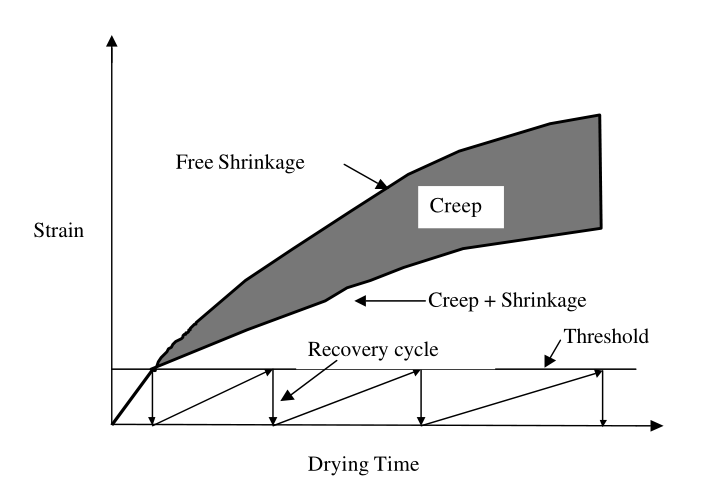
\includegraphics[width=.5\linewidth]{aci1}
  \caption{Schematic diagram of the test mechanism \cite{cscea}.}\label{aci1}
\end{figure}

\subsection{Results}
According to the free shrinkage study, a first stage in which no shrinkage is
experienced by the concrete seems to occur, which is supposed to be caused by
evaporative cooling of the concrete specimens leading to a slight expansion of
the specimens. In the first 10 hours of the study, expansion or shrinkage could
occur depending on the sample.

The results also display a high shrinkage rate during the following 40 hours of
testing. The study of fiber-reinforced concrete showed that steel fibers did
not impact shrinkage, while the use of polypropylene fibers led to a small
increase of free shrinkage.

Although all restrained shrinkage specimens cracked, fracturing time varied
strongly among the different specimens. A lower rate of shrinkage was observed
for higher water to cement ratio, causing longer fracturing times. Steel
fiber reinforced specimens also showed delayed fracturing for all water to
concrete ratios, with more higher delays for low water to cement ratios. By
contrast, polypropylene fibers caused earlier failure due to the shrinkage
behavior observed before.

According to the findings of this study, other factors than tensile stress have
an importance in cracking behavior of restrained concrete. For instance,
high-performance concrete cracked earlier than normal concrete despite
sustaining the same tensile stress. Stress history has a strong influence on
the performance of the material regarding cracking. Other findings include that
the failing stress is not equal to the tensile strength of the material, and is
lower by around \SIrange{20}{25}{\percent}.

Relative humidity of the drying environment had an effect on the failing
stress, with lower relative humidities leading to earlier failures, but only
with normal concrete samples.

Creep also had a major impact on cracking by doubling the shrinkage capacity of
a given concrete element. The results highlight a creep to shrinkage ratio of
around \SI{50}{\percent}, with a rapid evolution during the first 2 days
stabilizing between \num{0.5} and \num{.6}. Fiber reinforcement had little
impact on the creep to shrinkage ratio.

An alternate drying/wetting experiment was also conducted and showed that the
wetting of the concrete led to a high shrinkage recovery rate. An important
note is that the shrinkage rate after a second drying was lower than after the
first continuous drying period. However, creep was also partly reduced by this
approach, and further investigation would be needed to fully understand the
effects of alternate drying and wetting of concrete elements.

\subsection{Conclusion}
The extensive experimental testing conducted for this research paper shows that
several components play a role in the forming of cracks in concrete at
early-age. The study highlights the crucial role of stress rate and history on
the cracking stress and time. It also displays the importance of the actual
tensile strength, which is found to be lower than the usual static tensile
strength of the hardened concrete. Creep also has a major impact, and should be
considered in cracking studies. Curing practices also seem to have a notable
impact on cracking.

\section[State-of-the-Art Report on Control of Cracking in Early Age Concrete]
{State-of-the-Art Report on Control of Cracking in Early Age Concrete \cite{soa}}

\subsection{Introduction}
In 2003, a team of researchers wrote a state-of-the-art on cracking control in
concrete. The goal was to review research on the causes of cracking as well as
the methods that are used to control cracking of concrete.

\subsection{Causes of cracking}
According to this paper, three types of deformation are considered when
studying cracking. Autogenous shrinkage the volume reduction
caused by the hydration of cement in early-age concrete. Drying shrinkage is
created by the evaporation of the water present in early-age concrete. Finally,
thermal shrinkage represents the deformation caused by the changes in concrete
temperature during curing.

These deformation types have a different impact depending on the concrete type.
Low water to cement ratio concretes are more subjected to autogenous shrinkage, while
ordinary concretes tend to be more prone to drying shrinkage.

An important difference between autogenous and drying shrinkage is also the
fact that autogenous shrinkage tends to be uniform in a concrete element, while
drying shrinkage appears more prominently on the surface, leading to non-uniform
deformations.

Creep also plays a role in cracking by allowing a gradual relaxation of
stresses. The total strain would then be defined by \autoref{eq:1}:
\begin{equation}
  \epsilon_{\text T}(t) =
  \epsilon_{\text{elastic}}(t) +
  \epsilon_{\text{creep}}(t) +
  \epsilon_{\text{shrinkage}}(t) +
  \epsilon_{\text{thermal}}(t)
  \label{eq:1}
\end{equation}

In absence of external loading, this shows that cracking of early-age concrete
is caused by the presence of restraints on deformations of concrete elements.

\subsection{Material properties}
Since most material properties of concrete are rapidly evolving during the
curing process, it is crucial to establish accurate representation of these
characteristics in order to be able to study cracking accurately.

The elasticity of concrete changes rapidly during the first days of curing. It
only starts to show a similar behavior to hardened concrete after 14 hours.
It is also notable that the tensile elastic modulus is generally higher than
compressive elastic modulus by about \SIrange{10}{20}\percent.

Another point is that tensile creep differs in value from compressive creep,
with a ratio of around \SI{75}\percent between the specific tensile creep and
specific compressive creep.

Since thermal behavior also plays a role in cracking, it is important to
establish accurately the linear expansion coefficient at early-age. It has
proved difficult to isolate the thermal expansion coefficient from other
effects at early age, but it has been found that it is generally larger for
early age concrete than hardened concrete and that it varies greatly with time.

\subsection{Numerical models}

Several models have also been developed for concrete at early-age. For
instance, rheological models like the Burger's model displayed in
\autoref{burgers} have been used to represent the different strains that can
appear at early age.

\begin{figure}
  \centering
  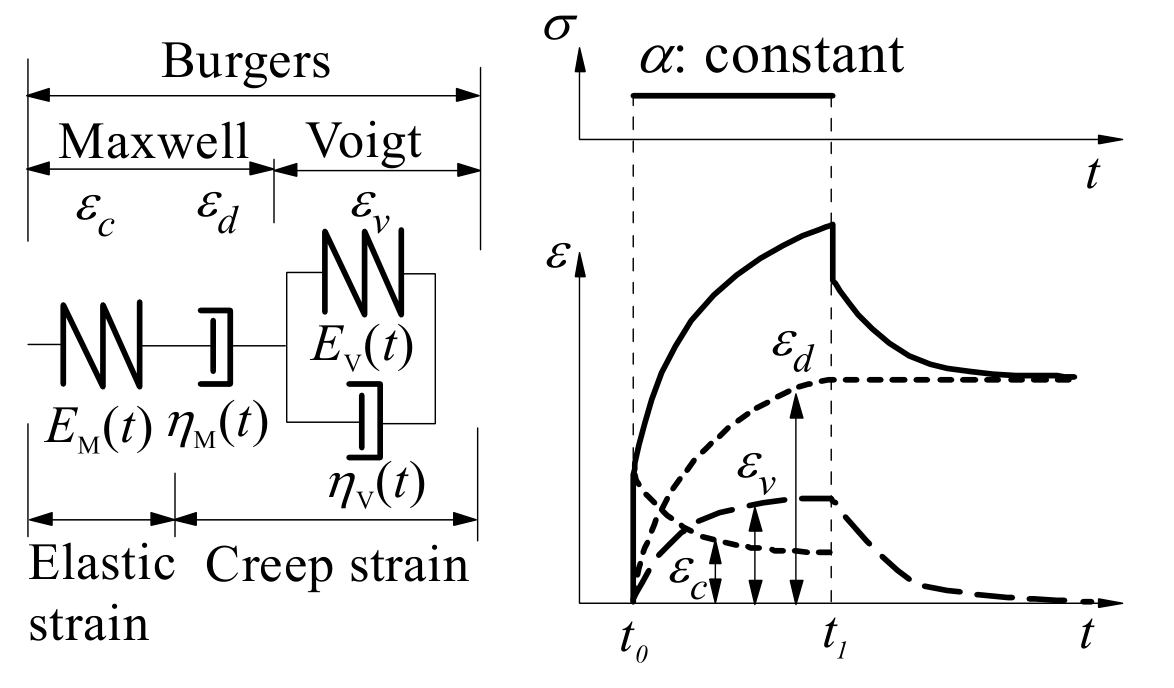
\includegraphics[width=.5\linewidth]{burgers}
  \caption{Schematic representation of Burgers model (Nakamura \textit{et al.}
  2002).}\label{burgers}
\end{figure}

\section{Comparison between standard methods for cracking risk evaluation}
\subsection{Introduction}

Several standard methods have been introduced by several institutes in order to
provide guidelines for designing concrete structures against cracking risk.

The Japan Concrete Institute released guidelines in 2012 \cite{jci}, while the
American Concrete Institute released a guide in 2001 \cite{aci}.

\subsection{Standard methods}

\subsubsection{JCI}
The JCI guidelines focus mainly on cracking caused by the hydration of cement,
which includes the volume change due to the temperature changes and due to
autogenous shrinkage.

A thermal cracking index is defined for cracking verifications:
\begin{equation}
  I_{cr} = \frac{f_t(t_e)}{\sigma_t(t_e)}
\end{equation}
Where $f_t$ is the tensile strength of the concrete and $\sigma_t$ is the
principal tensile stress.

In order for the cracking probability to be under \SI5\percent, a limit is
defined for the thermal cracking index:
\begin{equation}
  I_{lim} = 1.85
\end{equation}

In order to obtain accurate cracking indexes, the JCI recommends the use of
three-dimensional finite element method.

\subsubsection{ACI}

\begin{figure}
  \centering
  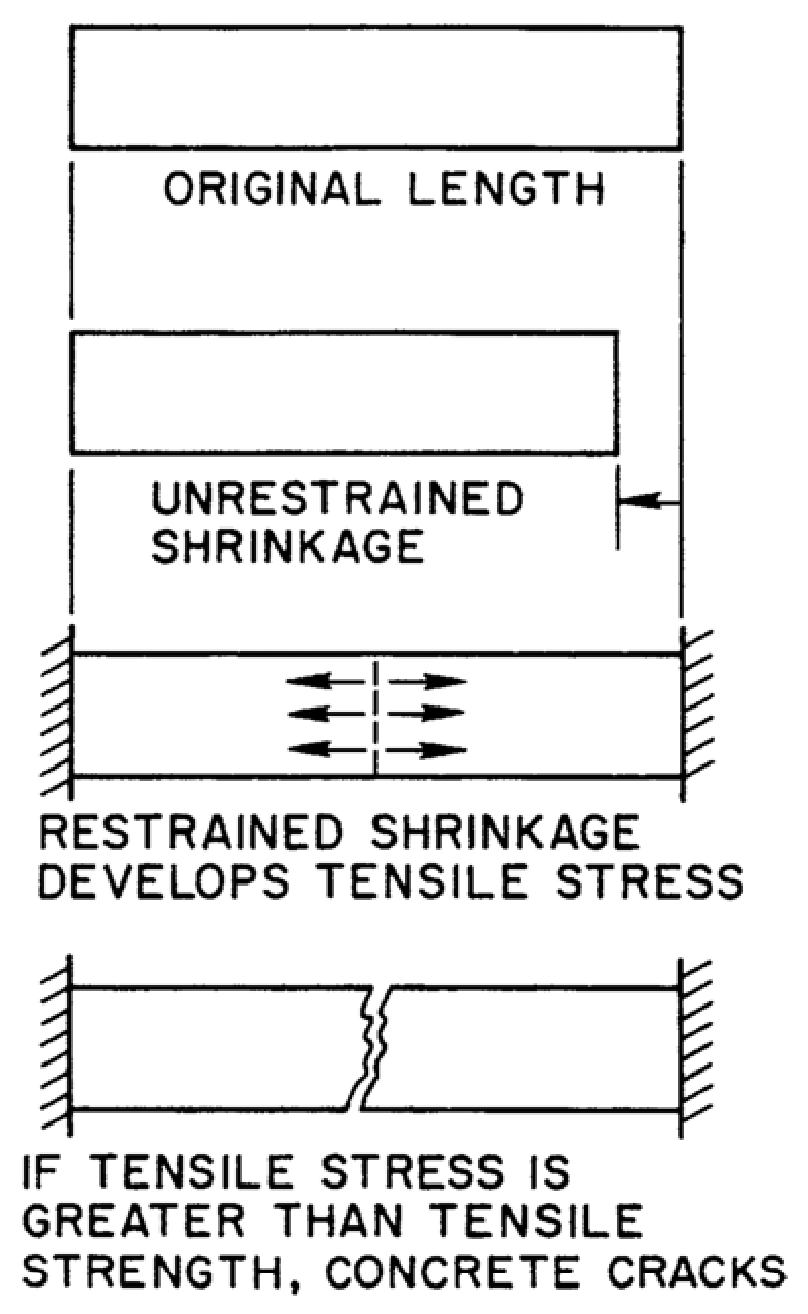
\includegraphics[width=.3\linewidth]{aci}
  \caption{Cracking of concrete due to drying shrinkage (ACI \cite{aci}).}\label{aci}
\end{figure}

The ACI's guidelines on cracking control are not as developed as other
institutes. The most notable part is that the maximum acceptable tensile stress
regarding the cracking risk is the tensile strength of the used concrete
(\autoref{aci}), with
no lowering factor added as in the JCI's guidelines for instance.

\subsection[Reliability of standard methods for evaluating the early-age
cracking risk of thermal-shrinkage origin in concrete walls]
{Reliability of standard methods for evaluating the early-age
cracking risk of thermal-shrinkage origin in concrete walls \cite{rsm}}
A study was conducted in 2019 on the reliability of existing guidelines
regarding the cracking risk in walls.

\subsubsection{Methods}
The study focused on validating the standard methods on two example walls,
which the researchers considered sufficiently different to allow for reliable
validation of the methods. Several parts of the guidelines were studied. Crack
width and spacing as well as temperature calculations are present but the focus
here will be rather on cracking risk.

\subsubsection{Results}
The findings of the study show that cracking risk was accurately predicted for
all methods, although this study does not primarily focus on the cracking risk
aspect of standard guidelines. In the studied scenarios, a remarkable remark is
that at early-age, shrinkage only has a minor effect compared to the thermal
effects that are happening simultaneously, with the resulting strain being
under \SI3\percent of the thermal strains.

\section{Conclusion}

From the existing research on cracking, it seems that the factors implicated in
the cracking of concrete elements are numerous. The most relevant phenomenons
leading to cracking are shrinkage, which can be separated in drying shrinkage
and autogenous shrinkage, and the thermal effects caused by the temperature
changes inside concrete elements. Creep has a major impact on reducing the
strains created by those factors, and should also be considered to prevent
major overestimations of the cracking risk.

All these factors are considered in the Eurocode~2, showing no major issue on
that first part. Nevertheless, it seems that strain history also has a major
impact on cracking, but is not considered in the calculations proposed in the
Eurocode~2.

Despite this shortcoming, comparative research has shown that the Eurocode~2's
method for evaluating cracking risk appears to be accurate.

It should also be noted that although the Eurocode~2 provides simplified
calculations for the cracking risk, the Japanese Concrete Institute advises to
use finite-element modeling to reach good accuracy, and the American guidelines
are even more simplified.

%%%
\backmatter
\printbibliography
\end{document}
